
\documentclass[12pt,twoside]{reedthesis}

\usepackage{graphicx,latexsym} 
\usepackage{amssymb,amsthm,amsmath}
\usepackage{longtable,booktabs,setspace} 
\usepackage{chemarr} %% Useful for one reaction arrow, useless if you're not a chem major
\usepackage[hyphens]{url}
\usepackage{rotating}
\usepackage{natbib}
% Comment out the natbib line above and uncomment the following two lines to use the new 
% biblatex-chicago style, for Chicago A. Also make some changes at the end where the 
% bibliography is included. 
%\usepackage{biblatex-chicago}
%\bibliography{thesis}

% \usepackage{times} % other fonts are available like times, bookman, charter, palatino

\title{My Final College Paper}
\author{Blake Rosenthal}

\date{May 2015}
\division{Mathematics and Natural Sciences}
\advisor{Albert Kim}

\department{Mathematics}
%\approvedforthe{Committee}

\setlength{\parskip}{0pt}

\begin{document}

  \maketitle
  \frontmatter % this stuff will be roman-numbered
  \pagestyle{empty} % this removes page numbers from the frontmatter

% Acknowledgements (Acceptable American spelling) are optional
% So are Acknowledgments (proper English spelling)
    \chapter*{Acknowledgements}
	I want to thank a few people.

% The preface is optional
% To remove it, comment it out or delete it.
    \chapter*{Preface}
	This is an example of a thesis setup to use the reed thesis document class.

    \tableofcontents
% if you want a list of tables, optional
    \listoftables
% if you want a list of figures, also optional
    \listoffigures

% The abstract is not required if you're writing a creative thesis (but aren't they all?)
% If your abstract is longer than a page, there may be a formatting issue.
    \chapter*{Abstract}
	The preface pretty much says it all.
	
	\chapter*{Dedication}
	You can have a dedication here if you wish.

  \mainmatter % here the regular arabic numbering starts
  \pagestyle{fancyplain} % turns page numbering back on

%The \introduction command is provided as a convenience.
%if you want special chapter formatting, you'll probably want to avoid using it altogether

    \chapter*{Introduction}
         \addcontentsline{toc}{chapter}{Introduction}
	\chaptermark{Introduction}
	\markboth{Introduction}{Introduction}
	% The three lines above are to make sure that the headers are right, that the intro gets included in the table of contents, and that it doesn't get numbered 1 so that chapter one is 1.

% Double spacing: if you want to double space, or one and a half 
% space, uncomment one of the following lines. You can go back to 
% single spacing with the \singlespacing command.
% \onehalfspacing
% \doublespacing
	
	
	
    \chapter{Kriging}
    	\section{Spatial statistics}
Kriging is a method utilized in the field of geostatistics to model spatial data. Originally developed from the South African mining industry in the 1950's \cite{cressie:1993}, kriging provided a way to predict ore-grade distributions based on a limited empirical sample. Though the name comes from mining engineer D. G. Krige, methods for optimal spatial linear prediction from Wold (1938), Kolmogorov (1941b), and Wiener (1949) all include the crucial covariance component of spatial interpolation, realizing that points closer to the prediction point should be given greater weights than further points. This is the cornerstone of the kriging method and is explored in detail in section 3. \\

Given a spatially continuous random process $Y(x)$ over some two-dimensional region $B$, a data sample $S_i: i=1, \dots, n$ is obtained from $Y$ at locations $x_i: i=1, \dots, n$. \footnote{A note on notation: here, $x$ will be used to specify a generic point in $Y$, while $\mathbf{s}$ will be used to indicate the vector of spatial coordinates or other dependent variables that make up the sample $S$.}From a practical perspective, $Y$ can be thought of as an underlying but unknown distribution of a variable of interest over $B$, be it ore-density, mineral concentrations, elevation, etc. $S$ is therefore a set of vectors containing an independent spatial component and a dependent variable or variables. Since $S$ is only a small and incomplete realization of the field $Y$, the standard geostatistical approach is to impose an underlying structure to the field consisting of a mean function $\mu(\mathbf{s})$ and a random error process with zero mean $e(\mathbf{s})$. Together these specify that 

\begin{align*}
Y(\mathbf{s}) = \mu(\mathbf{s}) + e(\mathbf{s}),
\end{align*}

where $\mu(\mathbf{s}) = E[Y(\mathbf{s})]$.
  \\

The goal is to make some predictions regarding the underlying random process $Y$. Kriging at its simplest is a matter of predicting a value of $Y(x_i)$ at an arbitrary point within the region $B$. \emph{Simple kriging} assumes $Y$ to have a constant mean which is estimated from the sample mean of $S$. \emph{Ordinary kriging} uses the estimated covariance structure of $Y$ to replace the sample mean with the generalized least squares estimate of $\mu$. Finally, \emph{universal kriging} uses a trend surface model for the mean. 

\section{Estimation of the mean function}

Simple, ordinary, and universal kriging all differ in their approach to estimating the mean function. Simple kriging, which assumes a constant mean, is typically dismissed by most statisticians since it usually fails to accurately describe any naturally occurring random process. Here we go over universal kriging since it is the best linear unbiased prediction model for geostatistical random fields \cite{gelfand:2010}. \\

The purpose of the mean function is to help provide an estimate for the residuals $e(\mathbf{s})$, given by $\hat e$. This estimate is then used to calculate the semivariogram, described in the following section, which is then used in the universal-kriging equations. The mean function is given by $\mu(\mathbf{s}) = E[Y(\bold{s})]$ and is modeled as the linear equation

\begin{align*}
\mu(\mathbf{s}; \mathbf{\beta}) = \mathbf{X}(\mathbf{s})^T \mathbf{\beta}
\end{align*} 

where $\mathbf{X}(\mathbf{s})$ is a vector of covariates observed at $\mathbf{s}$ and $\mathbf{\beta}$ is an unrestricted parameter vector. These variables could be simply latitude and longitude coordinates, but may also include such information as elevation, slope, windspeed, etc. If using only latitude and longitude, for example, a first order  trend surface model is given by

\begin{align*}
\mu(\mathbf{s}; \mathbf{\beta}) = \beta_0 + \beta_1s_1 + \beta_2s_2
\end{align*} 

where $\mathbf{s} = (s_1, s_2)$ are latitude and longitude. This definition, however, is not invariant to the choice of origin or orientation of the coordinate system \cite{gelfand:2010} and higher-order polynomials such as the quadratic allow for omnidirectional prediction calculations.

%\begin{align*}
%\mu(\mathbf{s}; \mathbf{\beta}) = \beta_0 + \beta_1s_1 + \beta_2s_2 + \beta_{11}s_1^2 + \beta_{12}s_1s_2 + \beta_{22}s_2^2.
%\end{align*} 

At this point the provisional linear mean function is then fitted to the available data. There are many ways to do this, but the ordinary least squares method is typically used. This method yields an estimator $\hat\beta_{OLS}$ given by 

\begin{align*}
\hat\beta_{OLS} = (\mathbf{X}^T\mathbf{X})^{-1}\mathbf{X}^T\mathbf{Y} 
\end{align*} 

where $\mathbf{X} = [X(\mathbf{s}_1), X(\mathbf{s}_2), \dots, X(\mathbf{s}_n)]^T$ and $\mathbf{Y} = [Y(\mathbf{s}_1), Y(\mathbf{s}_2), \dots, Y(\mathbf{s}_n)]^T$. \footnote{Equivalently, and perhaps easier to work with, $\hat\beta_{OLS} = \text{argmin}\sum_{i=1}^n[Y(\mathbf{s}_i) - \mathbf{X}(\mathbf{s}_i)^T\mathbf{\beta}]^2$.} \\

It is possible to stop the analysis here, but once we have the second-order dependency structure of the semivariogram from the following section we can reestimate the mean function using estimated generalized least squares. A method given by Zimmerman and Stein (\cite{gelfand:2010}, p. 40) involves estimating a covariance matrix to include in the mean estimation. The updated mean function can be then used to recalculate the residuals $\hat e(\mathbf{s})$ for the semivariogram.


\section{Covariance and the variogram}
Part of the effectiveness of the kriging method comes from the recognition that the data from a spatial sample are correlated based on proximity. Points closer together are expected to be more highly correlated than points with greater spatial separation. The variogram, or semivariogram, plots this correlation as a function of distance, and the empirical semivariogram is the observed covariance structure of the data \cite{gelfand:2010}. Given this, the semivariogram is defined by $\gamma(x_i - x_j) = {1\over 2} \text{var} \{ e(x_i) - e(x_j) \}$, for all $x_i, x_j \in B$. Intuitively, the semivariogram provides a way to visualize the correlative effects of distance on the sampled data. For example, given a set of locations in the Cartesian plane, points with no separation distance could be expected to have zero variation in their dependent variables, while the variance between very distant points can be expected to be much higher [Fig. \ref{fig:semivariogram}]. \\

\begin{figure}[h]
    \centering
    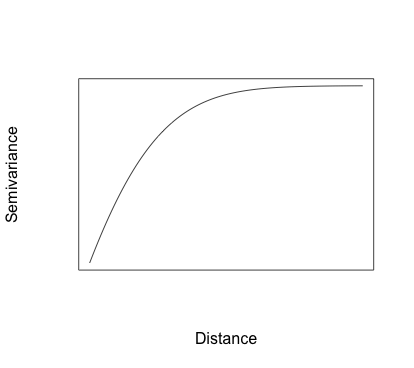
\includegraphics[width=0.8\textwidth]{semivariogram}
    \caption{An exponential semivariogram}
    \label{fig:semivariogram}
\end{figure}

The distance between any two points $x_i$ and $x_j$ can be can be used to define a new set $H = \{ x_i - x_j: x_i, x_j \in B \}$ for the continuous distribution of distances, or lags, in $B$. Elements of $H$ can be grouped into bins $H_1, H_2, \dots, H_k$. A representative lag for the entire bin $\mathbf{h}_u$ can be used to define the unbiased estimator of $\gamma(\bold{h}_u)$ by

\begin{align*} 
   \hat\gamma(\bold{h}_u) = { 1 \over {2n(H_u)}} \sum_{x_i - x_j \in H_u} [ \hat e(x_i) - \
   \hat e(x_j) ] ^2 \quad (u = 1, \dots, k)
\end{align*}

\noindent where $n(H_u)$ is the number of lags within the bin $H_u$ and $\hat e(x_i)$ is the residual at point $x_i$ after estimating the mean. This assumes that covariance between data points is a function of spatial distance only, and not location or other factors. This estimation also requires a subjective choice in binning -- since any exact distance, or lag, between two points is unlikely to occur frequently within a sample, it is necessary to group distances into representative intervals, or bins. A common way to do this is to make this binning choice up front, perhaps grouping the data into thirty or so bins then choosing $\mathbf{h}_u$ to be the average of all the lags that fall into a given bin. Therefore, unless the data is taken on a rectangular or polar grid, the accuracy of the semivariogram will always be dependent on the binning choices. What's the right number of bins? There's a trade-off -- more bins means that $\mathbf{h}_u$ is a better estimation of its representative bin $H_u$, yet there are fewer lags to any particular bin and a smaller sample size and therefore a greater sampling variation. This is an interesting optimization problem on its own, but the data itself may impose binning restrictions depending on the sample size and other factors. This means that there is therefore no uniquely optimized semivariogram. \\

Fitting a parametric model to the empirical variogram gives a convenient equation to work with for several reasons -- first, the empirical semivariogram will often have a high variance, and a smoothed version will have a lower variance that is easier to work with. Second, the empirical semivariogram usually fails to be conditionally nonpositive definite. This is a necessary condition when choosing predictors at later stages since the prediction error variance must be nonnegative at every point in the field. Third, predicting locations at lags not represented by the chosen bins requires a continuous function, something only a smoothed variogram can accomplish. This smoothed version must satisfy the following necessary and sufficient conditions to be a valid semivariogram: \\

\begin{enumerate}

\item Vanishing at 0: $\gamma(\bold{0}) = 0$
\item Evenness: $\gamma(-\bold{h}) = \gamma(\bold{h}$) for all $\bold{h}$
\item Conditional negative definiteness: $\sum_{i=1}^n \sum_{j=1}^n a_i a_j \gamma(x_i - x_j) \leq 0$ for all $n$, all $s_1, \dots, s_n$ and all $a_1, \dots, a_n$ such that $\sum_{i=1}^n a_i = 0$

A crucial assumption is that a ``true'' semivariogram exists for the entire region. By modeling the empirical semivariogram and fitting it to a curve we are guessing at the underlying model that represents the entire process. In a way, this describes the entire study of statistics in general: using incomplete data to make an educated guess about the underlying, inherently unknowable, system and adjusting to the model to minimize inaccuracies.

\end{enumerate}



\section{Spatial Prediction: Kriging}
Given a prediction point $\mathbf{s}_0$ \footnote{Usually this is an unknown point in $B$, but can also be a known point.}, the goal of kriging is to find a predictor $\hat Y(\mathbf{s}_0)$ for $Y(\mathbf{s}_0)$ that minimizes the prediction error variance $\text{var}[\hat Y(\mathbf{s}_0) - Y(\mathbf{s}_0)$ of all possible predictors that are both (1), linear, and  (2) unbiased:

\begin{enumerate}
\item $\hat Y(\mathbf{s}_0) = \mathbf{\lambda}^T\mathbf{Y}$, where $\mathbf{\lambda}$ is a vector of fixed constants and $\sum \lambda_i = 1$. 
\item $E[\hat Y(\mathbf{s}_0)] = E[Y(\mathbf{s}_0)]$, or equivalently, $\mathbf{\lambda}\mathbf{X} = \mathbf{X}(\mathbf{s}_0)$.
\end{enumerate}

Here $\lambda$ can be thought of as a vector of weights applied to the sample data. Since the value of $Y$ at $\mathbf{s}_0$ depends solely on the empirical data, optimizing this linear predictor with respect to the given restraints gives a unique solution. If $\lambda$ is a solution to this problem, then $\lambda^T\mathbf{Y}$ is a best linear unbiased predictor (BLUP) for $Y(\mathbf{s}_0)$. Here ``best'' means having the smallest mean squared error within the class of linear unbiased predictors. There are several ways of solving this. Cressie \cite{cressie:1993} gives a proof using differential calculus and Lagrange multipliers, while Zimmerman and Stein \cite{gelfand:2010} give a geometric proof. Both give the following solution:

\begin{align*}
\hat Y(\mathbf{s}_0) = [\gamma + \mathbf{X}(\mathbf{X}^T\Gamma^{-1}\mathbf{X})^{-1}(\mathbf{x}_0 - \mathbf{X}^T\Gamma^{-1}\gamma)]^T\Gamma^{-1}\mathbf{Y}
\end{align*}

where $\gamma = [\gamma(\mathbf{s}_1 - \mathbf{s}_0), \dots, \gamma(\mathbf{s}_n - \mathbf{s}_0)]^T$, $\Gamma$ is the $n \times n$ symmetric matrix with $ij$th element $\gamma(\mathbf{s}_i - \mathbf{s}_j)$ and $\mathbf{x}_0 = \mathbf{X}(\mathbf{s}_0)$. \\

Minimizing the prediction error variance then gives us the kriging variance which can be expressed as

\begin{align*}
\sigma^2(\mathbf{s}_0) = \gamma^T\Gamma^{-1}\gamma - (\mathbf{X}^T\Gamma^{-1}\gamma - \mathbf{x}_0)^T(\mathbf{X}^T\Gamma^{-1}\mathbf{X})^{-1}(\mathbf{X}^T\Gamma^{-1}\gamma - \mathbf{x}_0).
\end{align*}



\chapter{Oregon Water Data}

\section{Background}
A wide variety of data can be used for kriging, provided it meets a few necessary conditions. Most importantly, the data must be a sample from a spatially continuous random process. Since kriging provides a point prediction for any location within a region, a discrete or discontinuous random process cannot be used. \\

This thesis will analyze Oregon ground water depth using data from Oregon's Water Resources Department. The data itself is a collection of logs recorded by Oregon-bonded well drillers and includes such information as the drilling date, the depth of the well, the depth of the first occurrence of water, and flow rate. The Water Resources Department uses this data to monitor water quality throughout the state of Oregon. For the purposes of this thesis, the data represents a partial sampling from a mostly continuous supply of subterranean water. By applying kriging to the available sample, it is possible to make predictions for unsampled locations in Oregon. \\


\subsection{The Data}

Oregon's records contain nearly 500,000 wells in the state. Since the individual contractors are responsible for recording their own observations, much of the data is incomplete. Only a handful of the observations include the latitude and longitude coordinates necessary for spatial prediction. Of this subsample, a ten-year date window was selected for the sake of accuracy. \\

In addition to this, a few other error-correction edits were made to the data. Several lat/long locations placed points off the coast and theses were removed from the sample. The presence of these points may indicate a larger trend of recording errors among inland points, but since determining this error would be nearly impossible, the recorded values were taken for face value in the initial stages. The kriging process, however, does give some options for accounting for error and this is explored later. \\

Another edit made to the data was removing co-located points. Several points (n=15) had the same lat/long entries but different recorded depth values. While these points could be used to calculate the variogram's nugget effect, their relatively rare frequency taken with the already established recording errors found in the sample warranted their exclusion. 

\begin{table}[h!]

	\centering
	

 \begin{tabular}{l|l|l}

\hline
 Longitude &       Latitude &     Depth\\
\hline
 Min.   :-124.5   & Min.   :42.00   & Min.   :   0.0  \\
\hline
 1st Qu.:-123.2   & 1st Qu.:42.94   & 1st Qu.:  30.0  \\
\hline
 Median :-122.9   & Median :43.97   & Median :  82.0  \\
\hline
 Mean   :-122.1   & Mean   :43.81   & Mean   : 134.4  \\
\hline
 3rd Qu.:-121.5   & 3rd Qu.:44.67   & 3rd Qu.: 172.0  \\
\hline
 Max.   :-116.9   & Max.   :46.23   & Max.   :1000.0  \\
\hline



\end{tabular}
\label{data}
\caption{Summary of groundwater data variables}

\end{table}

Table \ref{data} gives a few preliminary stats on the data. The longitude and latitude variables correspond loosely with Oregon's bounding perimeter, and the depth values range from zero to 1000 feet. Figure \ref{depths} shows the frequency of recorded depths across all observations. Of particular note is the high frequency of shallower ( $<100$ feet) wells across the state. \\

Finally, Figure \ref{points} plots all observations over a map of Oregon, with color corresponding to depth. The clustering along the West side of the state is due to statewide population densities, with more Oregon residents living near the I-5 highway that runs North/South from Washington to California. This clustering becomes important later when we look at the predicted kriging variances and the superimposed standard deviation map.

\begin{figure}[h!]
	   
	       \centering
	  
	    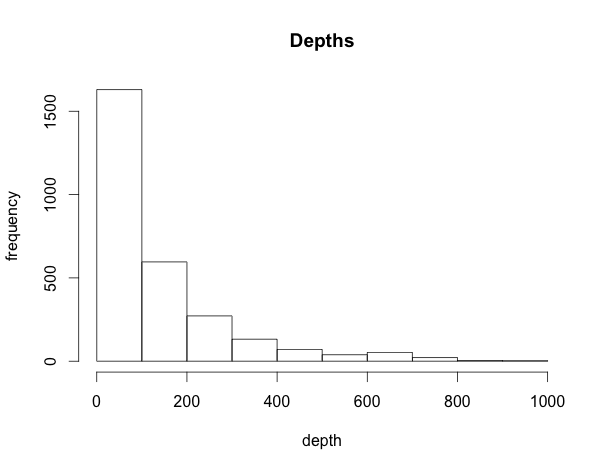
\includegraphics[scale=0.6]{depth_hist}
	
	     \caption{Depth frequency across data observations}
	 \label{depths}
	\end{figure}

\begin{figure}[h!]
	   
	       \centering
	  
	    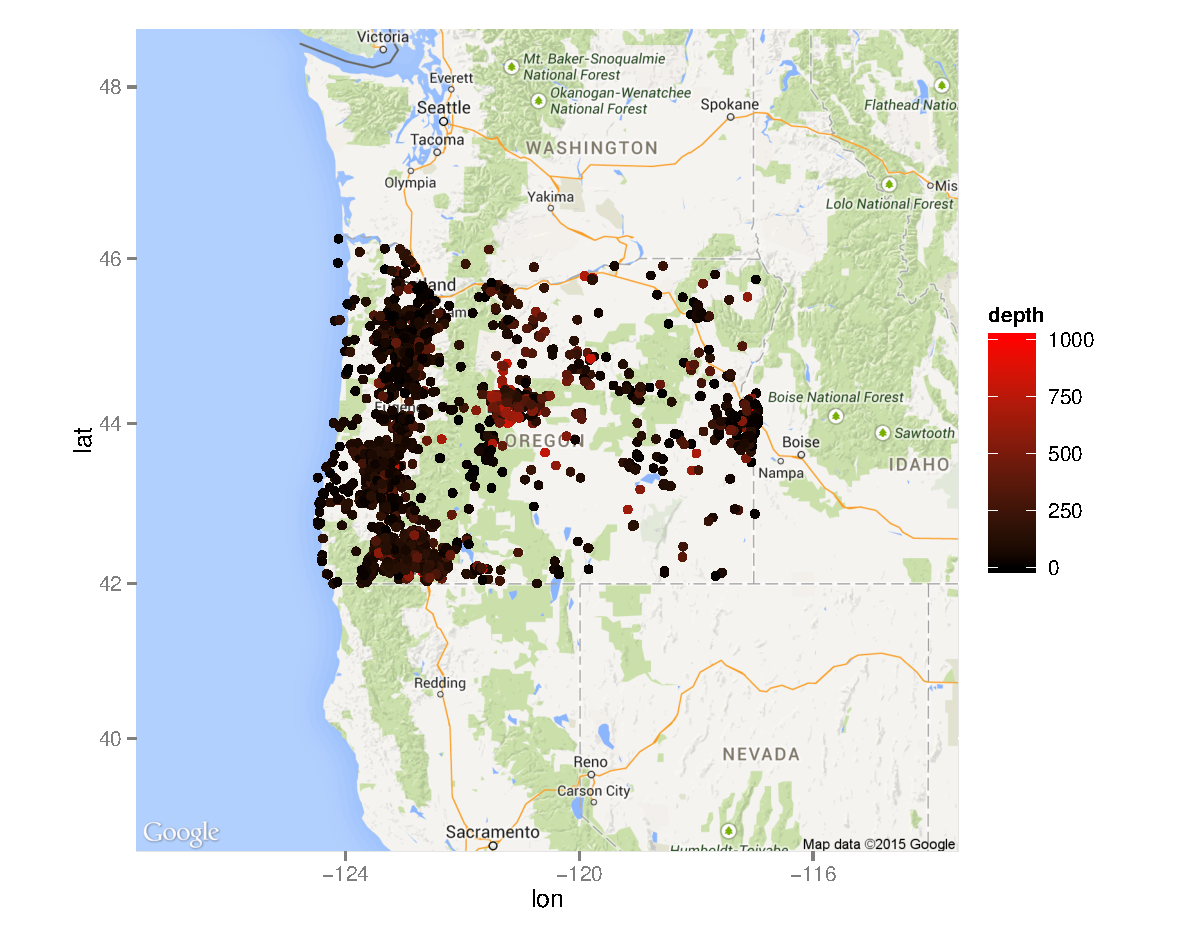
\includegraphics[scale=0.8]{points_plot}
	
	     \caption{Data observations with recorded depth values}
	 \label{points}
	\end{figure}


\section{The Variogram}


As described in section 1.3, the variogram plots the degree of correlation between points at varying distances. This correlation is then used to predict a depth at an unsampled location ($\mathbf{s}_0$) by comparing its distance to known locations to the lags associated with those distances. The degree to which the relative lags agree on the predicted value of $\mathbf{s}_0$ then determines the kriging variance. \\

Several choices go into the process of plotting the variogram. First, an effective range must be established in order to determine the maximum separation distance that will be used for the calculation. As shown in Table \ref{dists}, the average distance between data points is 237.8 kilometers while the maximum is 719 kilometers. For this reason, setting the maximum variogram distance to 300 kilometers as in Figure \ref{variogram} cuts out a lot of noise from distant and unrelated pairs while still including as many pairs as possible. 

\begin{table}[h!]

\centering

\begin{tabular}{l|l|l|l|l|l}

\hline
Min.  & 1st Qu.  & Median  &   Mean  & 3rd Qu.  &   Max. \\
\hline
  0.0007 & 118.3000 & 209.1000 & 237.8000 & 330.0000 & 719.0000 \\
\hline

\end{tabular}

\caption{Cartesian distances across data in kilometers}
\label{dists}

\end{table}
The second main choice is how many bins to choose. Again, the tradeoff between more or fewer bins is accuracy vs. variance. More bins means a greater number of distances is represented in the variogram, and fewer bins means each bin has a lower sampling variation. In most geostatistical applications, anywhere between 10 and 30 bins is typically used. For the purposes of the Oregon groundwater data, a binning number of 15 allows for 20 kilometers of separation between lags and between 115,000 and 240,000 pairs per bin. \\

The third necessary decision is whether to modify the data to represent accurate spatial distance. Since latitude and longitude are a two-dimensional projection on a curved surface, latitudes are equidistant, but the distances between longitudes varies\footnote{\cite{SpatialEpi}}. Because of this, distances between two points, $(x_1, y_1)$ and $(x_2, y_2)$, will not be accurate with respect to Euclidian distance, $d = \sqrt{(x_2 - x_1)^2 + (y_2 - y_1)^2}$. Converting to a grid-based coordinate system solves any problems this may cause. 


\begin{table}[h!]

\centering

\begin{tabular}{r|r|r}
\hline
Lag distances & lag & \# of pairs\\
\hline
20 & 11948.97 & 114487\\
\hline
40 & 15098.10 & 171869\\
\hline
60 & 14260.73 & 175836\\
\hline
80 & 13820.19 & 166287\\
\hline
100 & 14267.44 & 175306\\
\hline
120 & 16011.45 & 168228\\
\hline
140 & 17206.47 & 183247\\
\hline
160 & 28851.95 & 200061\\
\hline
180 & 31363.58 & 234284\\
\hline
200 & 36084.79 & 226972\\
\hline
220 & 38299.19 & 199070\\
\hline
240 & 38914.69 & 174760\\
\hline
260 & 35559.17 & 179645\\
\hline
280 & 29084.78 & 172046\\
\hline
300 & 24320.69 & 153338\\
\hline
\end{tabular}

\caption{Variogram binning}
\label{bins}

\end{table}

Table \ref{bins} shows the total number of pairs and variances for each bin. When plotted as in Figure \ref{variogram}, we see a trend similar to that in Figure \ref{fig:semivariogram}. This is the empirical semivariogram and is the foundation for the fitted model.
	
\begin{figure}[h!]
	   
	       \centering
	  
	    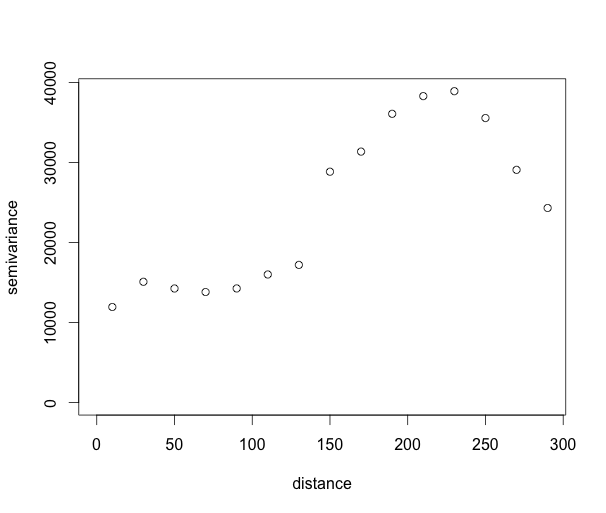
\includegraphics[scale=0.6]{Variogram}
	
	     \caption{Empirical variogram with 300 km maximum distance}
	 \label{variogram}
	\end{figure}

\subsection{Fitting a model}

Variograms in general tend to increase roughly with distance. Because of this, the most common fitted models are ones that increase monotonically, but this is not a necessary condition. Any model must meet the three conditions from Chapter 1, namely 1) vanishing at zero, 2) evenness, and 3) conditional negative definiteness. The most common tends to be the Mat\'ern model, given by 

\begin{align*}
\gamma(h) = \theta_1\left (1-{{(h/\theta_2)^\nu\kappa_{\nu}(h/\theta_2)}\over{2^{\nu-1}\Gamma(\nu)}} \right )
\end{align*}

where $\kappa_\nu$ is the modified Bessel function of the second kind of order $\nu$ (\cite{gelfand:2010}) and $(\theta_1, \theta_2)$ is a parameter vector to be optimized. \\

Figure \ref{matern} shows the empirical variogram from Figure \ref{variogram} fitted with a Mat\'ern model. The fit was calculated using Weighted Least Squares (WLS) given by

\begin{align*}
\hat{\mathbf{\theta}} = \text{argmin}\sum_{h \in H_u} {{n(\mathbf{h}_u)}\over{[\gamma(\mathbf{h}_u)]^2}}[\hat\gamma(\mathbf{h}_u) - \gamma(\mathbf{h}_u)]^2
\end{align*}

with all variables defined as in Chapter 1. Note that either a large $\gamma(\mathbf{h}_u)$ or a small $n(\mathbf{h}_u)$ corresponds to smaller weights. This means that larger lags are given less weight than smaller lags. \\

When choosing a model, a few particular attributes play an important role. Notably the \emph{sill}, \emph{range}, and \emph{nugget} of the model will significantly affect the kriging calculation. The sill is effectually the highest point in the variogram, or the maximum variance across all pairs of data points (i.e. $\text{lim}_{h\to\infty}\gamma(h)$ provided the limit exists). For the Mat\'ern model this corresponds with $\theta_1$. The range is the smallest value of $\mathbf{h}$ for which the variogram equals its sill. The nugget is defined as $\text{lim}_{h\to0}\gamma(h)$, or the y-intercept,  and can be thought of as a measurement error that accounts for differing data values at very close or co-located points. These three attributes are generally considered just as much as closeness-of-fit when choosing a variogram model. \\

In addition to the Mat\'ern model, several common functions include the exponential (Figure \ref{exp}), the power (Figure \ref{cubic}), and the spherical (Figure \ref{sph}). Table \ref{param} gives the optimized parameter vectors for each model as fitted to the empirical variogram from this section, with tau squared being the nugget variance, sigma squared the sill, and phi the range. Though all are good fits, the kriging step in the following section uses the spherical model, given by

\begin{align*}
\gamma(h) = \theta_1 \left ( {{3h}\over{2\theta_2}} - {{h^3}\over{2\theta_2^3}} \right )
\end{align*}

for $0 \leq h \leq \theta_2$ and 0 for $h > \theta_2$.

\begin{figure}[h!]
	   
	       \centering
	  
	    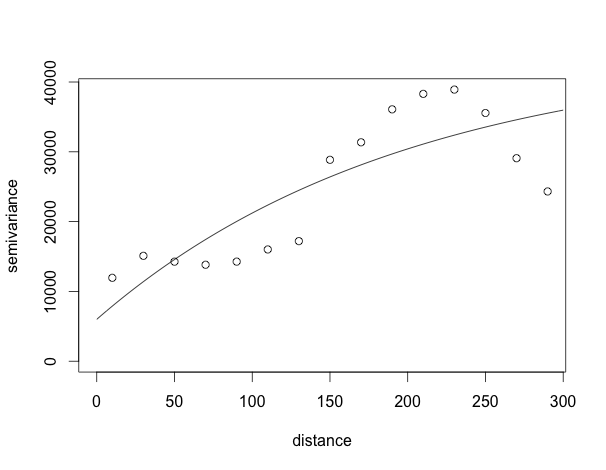
\includegraphics[scale=0.5]{vario_matern}
	
	     \caption{Empirical variogram with mat\'ern model}
	 \label{matern}
	\end{figure}
	
\begin{figure}[h!]
	   
	       \centering
	  
	    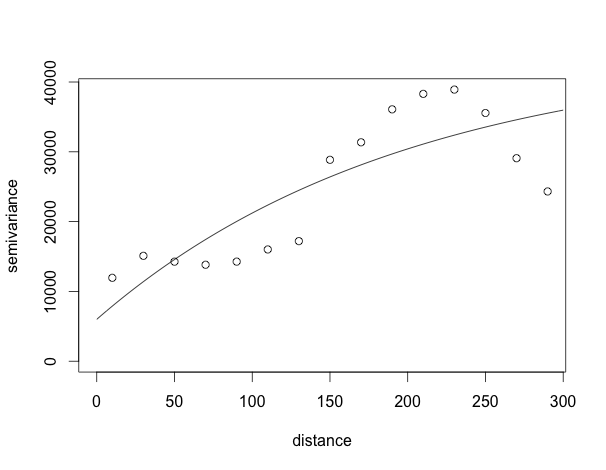
\includegraphics[scale=0.5]{vario_exp}
	
	     \caption{Empirical variogram with exponential model}
	 \label{exp}
	\end{figure}
	
\begin{figure}[h!]
	   
	       \centering
	  
	    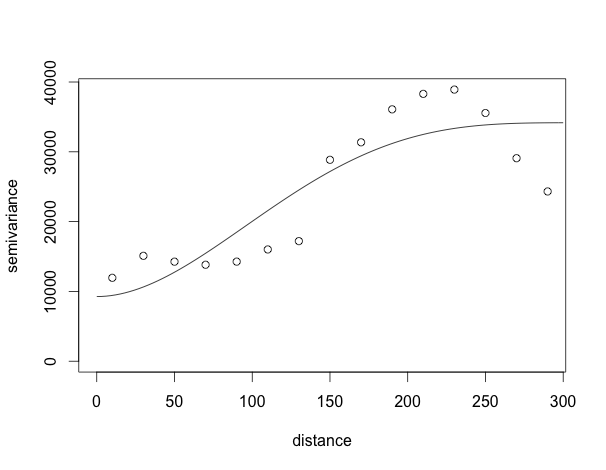
\includegraphics[scale=0.5]{vario_cubic}
	
	     \caption{Empirical variogram with cubic model}
	 \label{cubic}
	\end{figure}
	
\begin{figure}[h!]
	   
	       \centering
	  
	    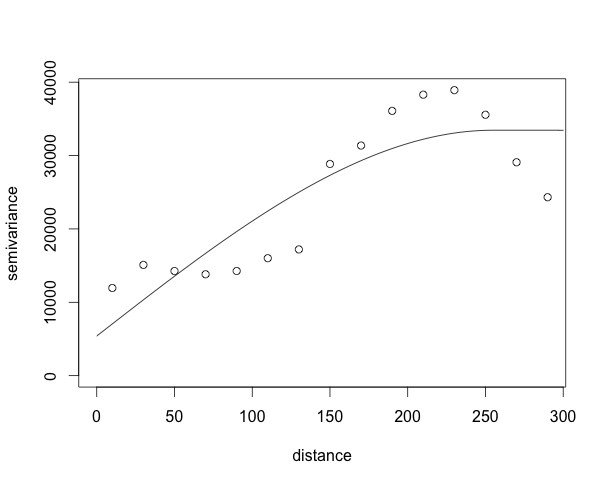
\includegraphics[scale=0.5]{vario_spherical}
	
	     \caption{Empirical variogram with spherical model}
	 \label{sph}
	\end{figure}
	
\begin{table}[h!]

\centering

\begin{tabular}{l|l|l}

\hline
 Spherical variogram &&\\
\hline
tau squared  &  sigma squared     &   phi \\
\hline
 5402.2780 & 28048.6894  & 254.8803 \\
 \hline \\
 \hline
 Mat\'ern variogram&& \\
\hline
 tau squared  & sigma squared   &    phi \\
 \hline
 6003.337 & 38428.555  & 198.255 \\
 \hline \\
 \hline
 Exponential variogram & &\\
\hline
 tau squared  & sigma squared   &    phi \\
 \hline
 6003.337 & 38428.555  & 198.255 \\
 \hline \\
 \hline
Cubic variogram & &\\
\hline
 tau squared &   sigma squared    &    phi \\
 \hline
 9260.4886 & 24906.8104  & 316.9988 \\
 \hline
 
 \end{tabular}
 
 \caption{Optimized parameters for several fitted variogram models}
 \label{param}
 
 \end{table}
 
 \section{Prediction}
 
 Once a working model has been established for the variogram, the prediction step is relatively straightforward. Using the equation from Chapter 1, and the variogram model from the previous section, we can define a grid of points over a prediction region and use it to build a topographical map. \\
 
 Figure \ref{grid} shows a grid of points constrained to the outer perimeter of Oregon. These will be the prediction locations for the kriging function. By further dividing the region into prediction blocks rather than points as in Figure \ref{tile}, it is possible to color each block with the prediction value associated with that block. 
 

 
 \begin{figure}[h!]
	   
	       \centering
	  
	    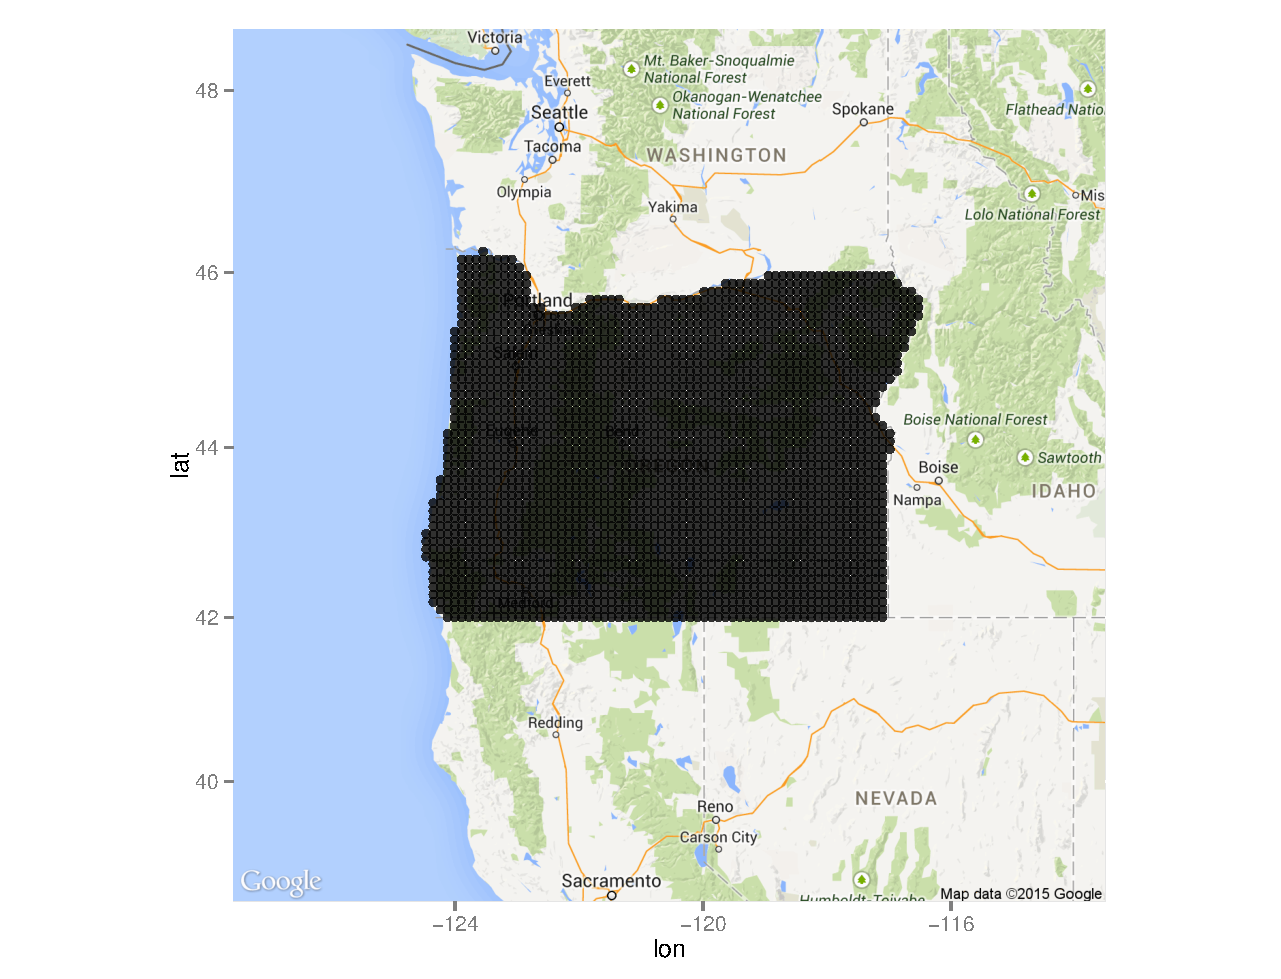
\includegraphics[scale=0.7]{pred_points}
	
	     \caption{Gridded prediction points}
	 \label{grid}
	\end{figure}
 
\begin{figure}[h!]
	   
	       \centering
	  
	    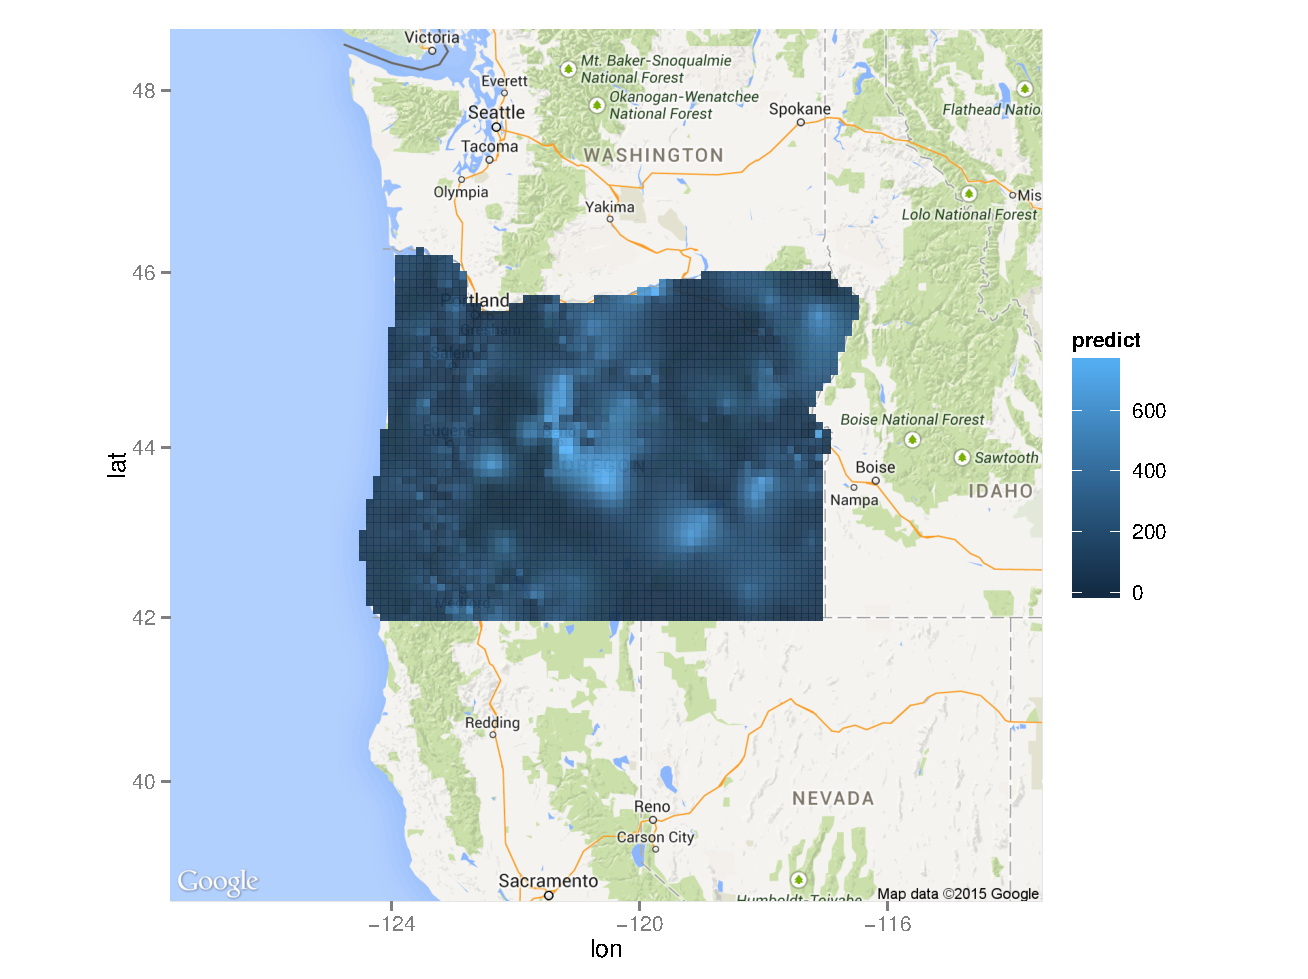
\includegraphics[scale=0.7]{tileplot}
	
	     \caption{Tiled prediction grid}
	 \label{tile}
	\end{figure}
	
\begin{figure}[h!]
	   
	       \centering
	  
	    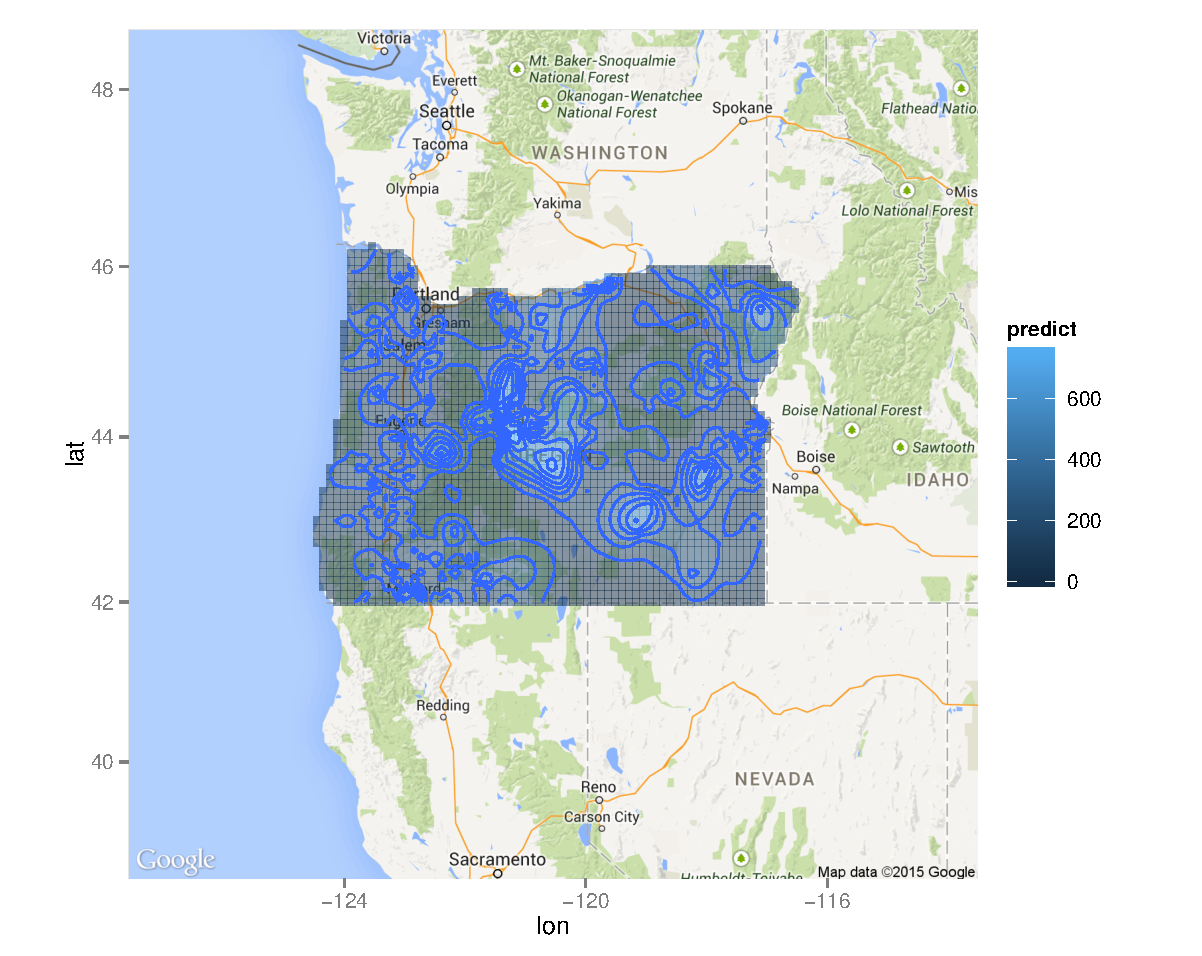
\includegraphics[scale=0.7]{contour_plot}
	
	     \caption{Prediction grid with contour lines}
	 \label{contour}
	\end{figure}
	
%\begin{figure}[h!]
	   
	   %    \centering
	  
	  %  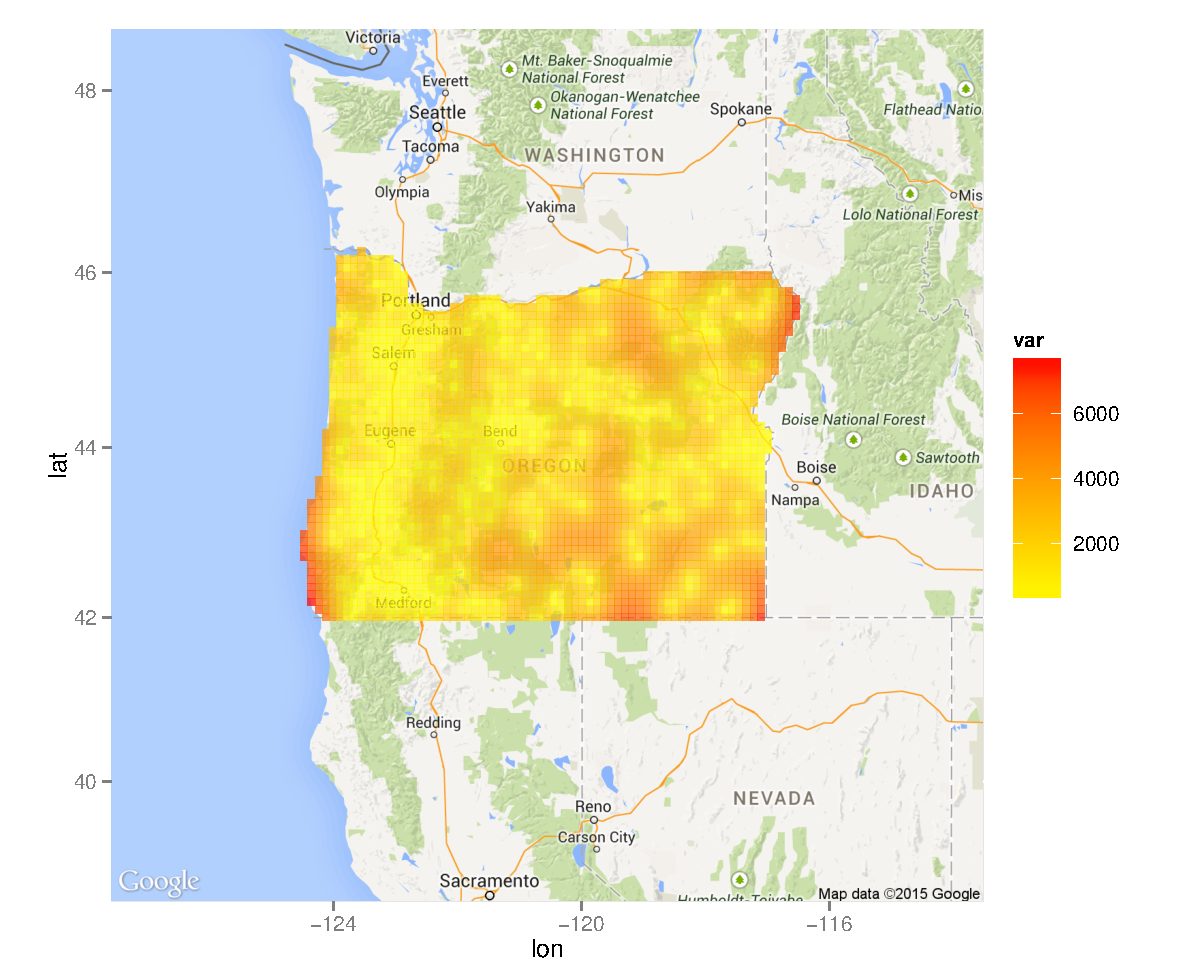
\includegraphics[scale=0.7]{var_plot}
	
	  %   \caption{Variance grid}
	% \label{var}
	%\end{figure}
	
\begin{figure}[h!]
	   
	       \centering
	  
	    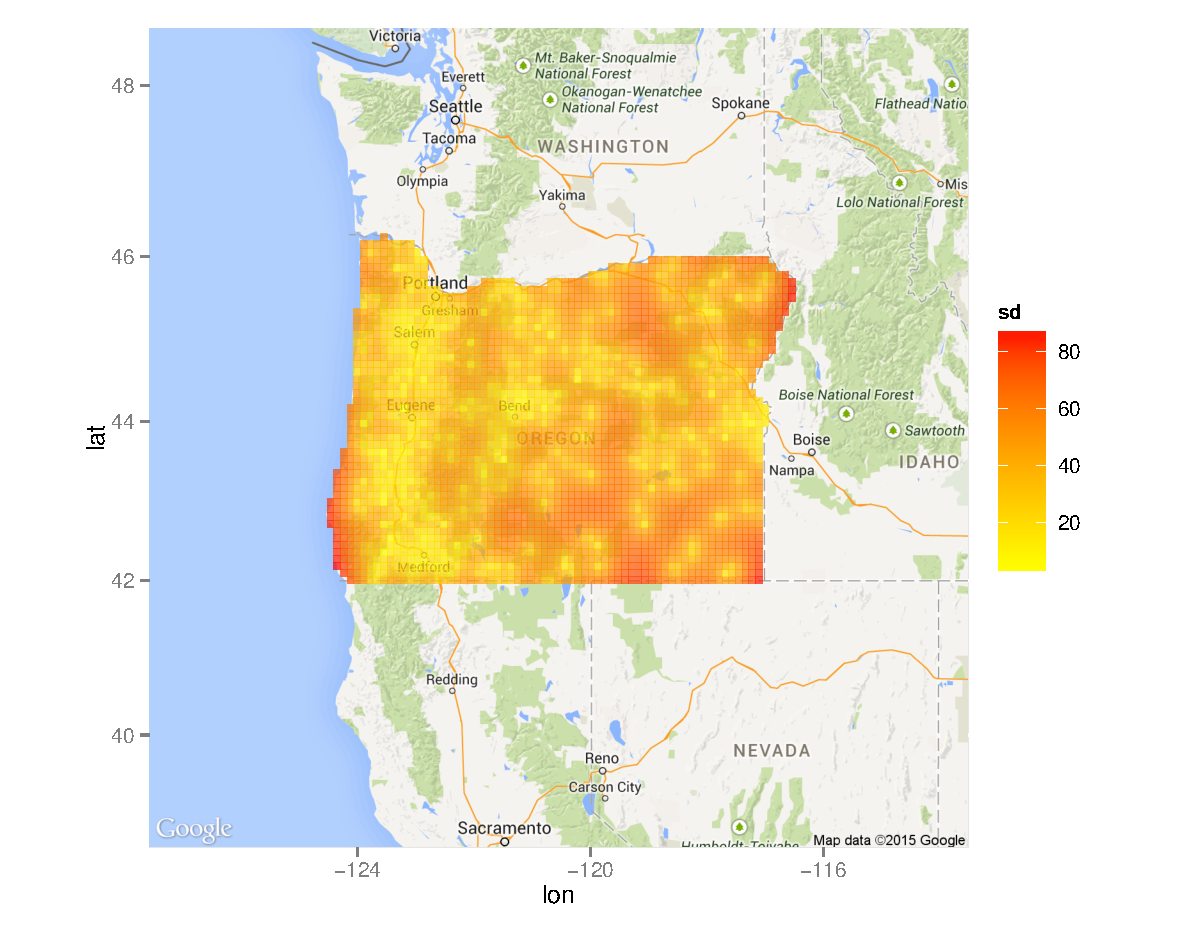
\includegraphics[scale=0.7]{sd_plot}
	
	     \caption{Standard deviation grid}
	 \label{sd}
	\end{figure}
	
%\begin{figure}[h!]
	   
	   %    \centering
	  
	   % 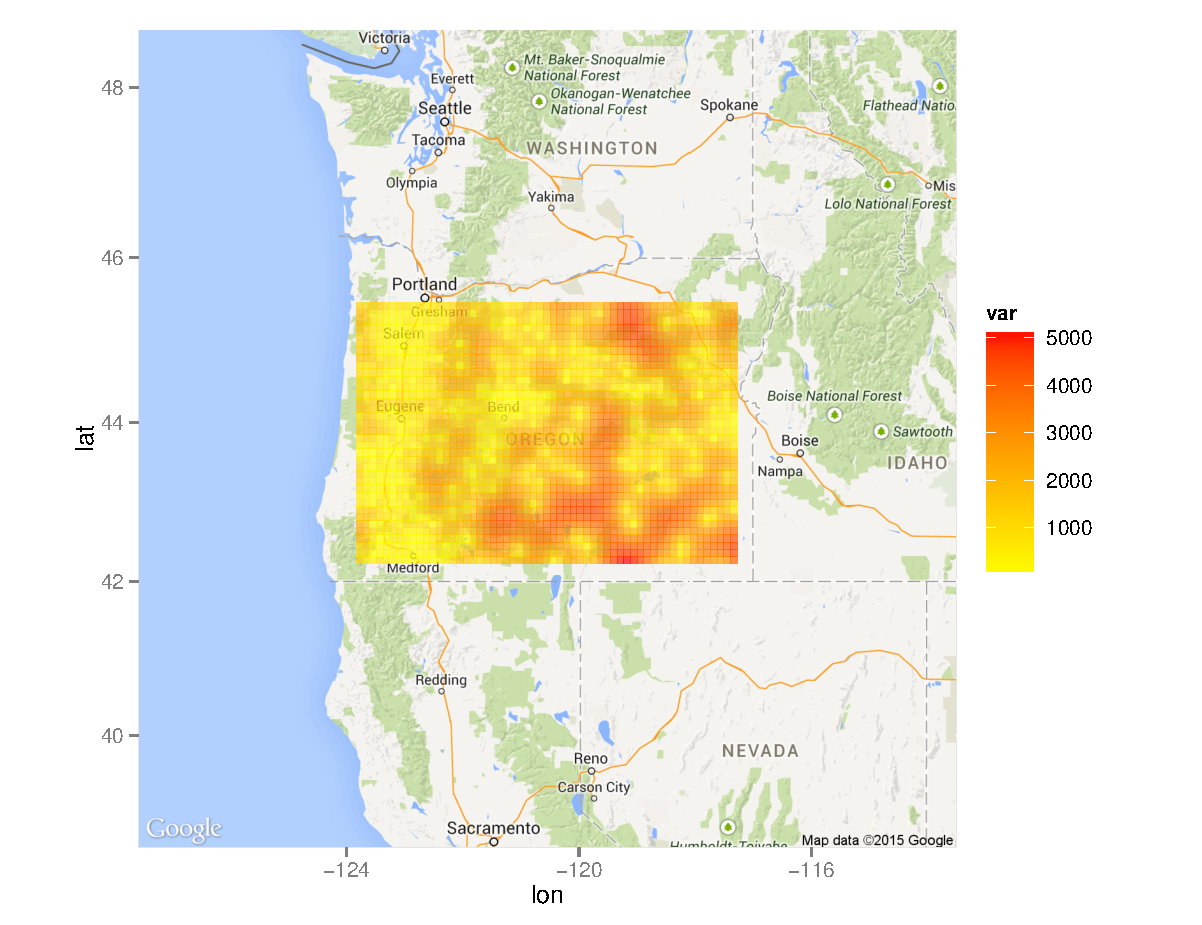
\includegraphics[scale=0.7]{var_crop}
	
	  %   \caption{Cropped variance plot}
	% \label{varcrop}
	%\end{figure}
	
\begin{figure}[h!]
	   
	       \centering
	  
	    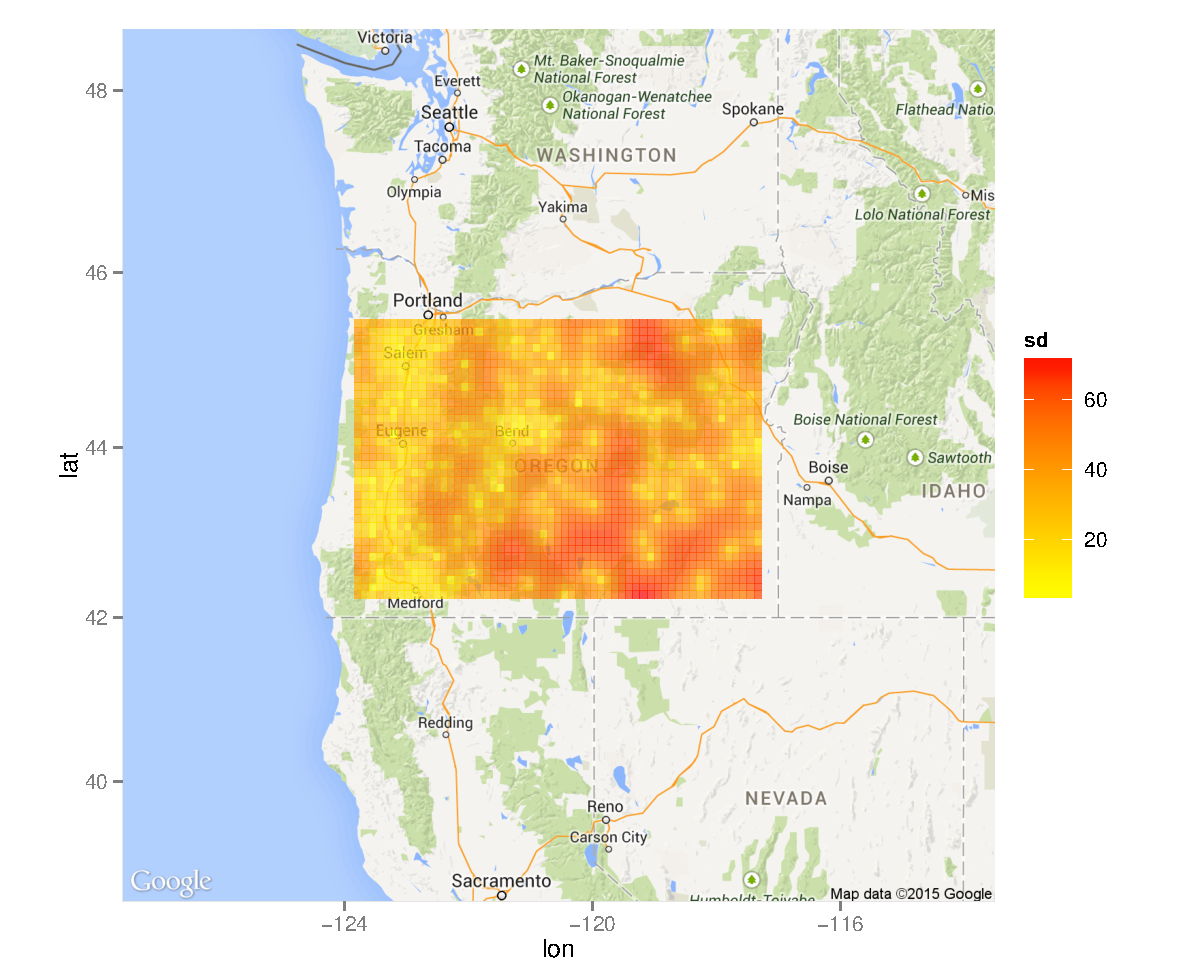
\includegraphics[scale=0.7]{sd_crop}
	
	     \caption{Cropped standard deviation plot}
	 \label{sdcrop}
	\end{figure}
	

\chapter*{Conclusion}
         \addcontentsline{toc}{chapter}{Conclusion}
	\chaptermark{Conclusion}
	\markboth{Conclusion}{Conclusion}
	\setcounter{chapter}{4}
	\setcounter{section}{0}
	



%If you feel it necessary to include an appendix, it goes here.
    \appendix
      \chapter{The First Appendix}
      \chapter{The Second Appendix, for Fun}


%This is where endnotes are supposed to go, if you have them.
%I have no idea how endnotes work with LaTeX.

  \backmatter % backmatter makes the index and bibliography appear properly in the t.o.c...

% if you're using bibtex, the next line forces every entry in the bibtex file to be included
% in your bibliography, regardless of whether or not you've cited it in the thesis.
    \nocite{*}

% Rename my bibliography to be called "Works Cited" and not "References" or ``Bibliography''
\renewcommand{\bibname}{Bibliography}

%    \bibliographystyle{bsts/mla-good} % there are a variety of styles available; 
%  \bibliographystyle{plainnat}
% replace ``plainnat'' with the style of choice. You can refer to files in the bsts or APA 
% subfolder, e.g. 
 \bibliographystyle{APA/apa-good}  % or
 \bibliography{kriging}
 % Comment the above two lines and uncomment the next line to use biblatex-chicago.
 %\printbibliography[heading=bibintoc]

% Finally, an index would go here... but it is also optional.
\end{document}
